% !TeX spellcheck = en_GB
% !TeX program = lualatex
%
% v 2.3  Feb 2019   Volker RW Schaa
%		# changes in the collaboration therefore updated file "jacow-collaboration.tex"
%		# all References with DOIs have their period/full stop before the DOI (after pp. or year)
%		# in the author/affiliation block all ZIP codes in square brackets removed as it was not %         understood as optional parameter and ZIP codes had bin put in brackets
%       # References to the current IPAC are changed to "IPAC'19, Melbourne, Australia"
%       # font for ‘url’ style changed to ‘newtxtt’ as it is easier to distinguish "O" and "0"
%
\documentclass[a4paper,
               %boxit,        % check whether paper is inside correct margins
               %titlepage,    % separate title page
               %refpage       % separate references
               biblatex,     % biblatex is used
               %keeplastbox,   % flushend option: not to un-indent last line in References
               %nospread,     % flushend option: do not fill with whitespace to balance columns
               hyphens,      % allow \url to hyphenate at "-" (hyphens)
               %xetex,        % use XeLaTeX to process the file
               %luatex,       % use LuaLaTeX to process the file
               ]{jacow}
%
% ONLY FOR \footnote in table/tabular
%
\usepackage{pdfpages,multirow,ragged2e,hyperref} %
%
% CHANGE SEQUENCE OF GRAPHICS EXTENSION TO BE EMBEDDED
% ----------------------------------------------------
% test for XeTeX where the sequence is by default eps-> pdf, jpg, png, pdf, ...
%    and the JACoW template provides JACpic2v3.eps and JACpic2v3.jpg which
%    might generates errors, therefore PNG and JPG first
%
\makeatletter%
	\ifboolexpr{bool{xetex}}
	 {\renewcommand{\Gin@extensions}{.pdf,%
	                    .png,.jpg,.bmp,.pict,.tif,.psd,.mac,.sga,.tga,.gif,%
	                    .eps,.ps,%
	                    }}{}
\makeatother

% CHECK FOR XeTeX/LuaTeX BEFORE DEFINING AN INPUT ENCODING
% --------------------------------------------------------
%   utf8  is default for XeTeX/LuaTeX
%   utf8  in LaTeX only realises a small portion of codes
%
\ifboolexpr{bool{xetex} or bool{luatex}} % test for XeTeX/LuaTeX
 {}                                      % input encoding is utf8 by default
 {\usepackage[utf8]{inputenc}}           % switch to utf8

\usepackage[USenglish]{babel}

%
% if BibLaTeX is used
%
\ifboolexpr{bool{jacowbiblatex}}%
 {%
  \addbibresource{ossym24.bib}
  \addbibresource{biblatex-examples.bib}
 }{}
\listfiles

%%
%%   Lengths for the spaces in the title
%%   \setlength\titleblockstartskip{..}  %before title, default 3pt
%%   \setlength\titleblockmiddleskip{..} %between title + author, default 1em
%%   \setlength\titleblockendskip{..}    %afterauthor, default 1em

\begin{document}

\title{A Dataset of GDPR Compliant NER\\ for Privacy Policies}

\author{Harshil Darji\thanks{Harshil.Darji@uni-passau.de}, Stefan Becher, Jelena Mitrovic,\\
        Armin Gerl, Michael Granitzer\\
        University of Passau, Passau, Germany}
	
\maketitle

%
\begin{abstract}
   Privacy policies play a vital role in informing users about the data practices of online platforms. They are intended to help them make informed decisions regarding the processing of their personal information. Still, privacy policies are often long and complicated, making it difficult for users to understand how their data is being handled. Natural Language Processing (NLP) techniques, such as Named Entity Recognition (NER), can be employed to automatically extract meaningful information from privacy policies to ease the making of informed decisions. In this work, we present a dataset of privacy policies improved with NER annotations. The dataset consists of privacy policies from 44 online platforms. These policies were annotated to comply with the GDPR guidelines. The privacy policies are manually annotated with NER tags, highlighting relevant entities of GDPR privacy policies such as data controllers, data sources, authority, etc. We also provide the annotation guidelines used by the annotators. This annotated dataset is a valuable resource for training and evaluating NER models in the context of privacy policies.
\end{abstract}


\section{Introduction}

In our digital age, data privacy has become a crucial issue due to the widespread use of online platforms \cite{6227909}. To safeguard individual rights and ensure transparent data handling, regulatory frameworks such as the General Data Protection Regulation (GDPR)\footnote{\url{https://gdpr-info.eu/}} have been implemented. An important GDPR compliance requirement is that organizations must provide concise, transparent, intelligible, and easily accessible privacy policies, using clear and plain language to inform users about the processing of their personal information. However, in reality, privacy policies are often extensive, complicated, and hard to understand \cite{9624976}, making it challenging for users to comprehend the data processing procedures. Thus, a gap between the regulatory requirements and the real-life implementation of privacy policies exists due to the necessity of presenting various and extensive information on the processing of personal data, which is clearly defined, while the communication and transparency requirements are only conceptually defined and, therefore, harder to implement. Therefore, there is a need for resources that can help bridge this gap and facilitate the understanding of privacy policies for non-expert readers.\\
The understanding of privacy policies is crucial to protecting personal information. Natural Language Processing techniques, especially Named Entity Recognition (NER), are instrumental in identifying entities within the text, such as \textit{Data subjects} and \textit{Personal Data entities} \cite{9582331}. However, NER has limitations in revealing complex document relationships and structures, which are essential for a thorough comprehension of privacy policies.

The GDPR policies on the web require in-depth statistical analysis. This evaluation helps users identify trustworthy policies and express their preferences. One way to improve this assessment may be to incorporate Relationship Extraction (RE). It has the potential to provide an in-depth analysis of the links between recognized entities, which can fill in any gaps left by NER. This approach can offer users a complete perspective of privacy policies.

% \textbf{\textit{Research goal:}} How can a dataset of GDPR-compliant privacy policies, annotated with NER tags, simplify the process of meeting GDPR transparency mandates? And, when leveraging this dataset, how do various language models compare in terms of accuracy and efficiency in their performance?

This paper aims to address this gap in research by introducing a GDPR-compliant privacy policy dataset that has been annotated with NER tags. The dataset comprises European privacy policies from various online platforms, annotated with NER tags to identify and highlight important entities within the policies, such as Data Controller, Data Processor, Data Source, etc.
 
The remainder of this paper is structured as follows: Section \nameref{section:related-work} studies the related research that displays the introduction and use of similar datasets. Section \nameref{section:dataset} introduces the dataset in question and also provides some statistics related to this dataset.

\section{Related work} \label{section:related-work}

The study presented in \cite{del2022systematic} aims to provide insights into the techniques used for extracting information from textual documents and their applications by conducting a systematic mapping study on the automated analysis of privacy policies. The study analyzed 39 papers out of 1097 publications, identifying the potential for extracting individual pieces of information from privacy policies. The research addresses the growing demand for automated privacy policy analysis across various stakeholders as well as the importance of understanding privacy concerns and complying with relevant data protection laws.

The research \cite{shankar2023privacyglue} proposes PrivacyGLUE, the first benchmark for measuring general language understanding in the privacy language domain, especially focusing on privacy policies. According to this study, privacy policies need a separate benchmark due to their distinct language. PrivacyGLUE comprises seven tasks related to privacy policies and evaluates the performances of five transformer language models. Similarly, to enhance the processing of legal texts, \cite{darji2023german} fine-tuned a German BERT model on a Legal Entity Recognition (LER) dataset \cite{leitner2019fine}, showing significant performance improvements over previous models and highlighting the importance of developing specialized models for legal documents to improve information extraction.


% Rel. Work regarding data sets
In the domain of data privacy, numerous datasets related to privacy policies have surfaced, requiring further studies.
\cite{opp115} created the OPP-115 data set, which is a collection of 115 manually annotated privacy policies, in 2016. 
Due to its creation date, the privacy policies the data set is based on are not compliant with the GDPR. 
There have been attempts to map the OPP-115 categories to GDPR articles to modernize the OPP-115 data set \cite{opp115-gdpr-mapping}. 
While this can create GDPR-compliant labels, it does not affect the outdated privacy policies as the basis of the data set. 
\cite{app350} annotated 350 mobile app privacy policies with privacy practices, which form the APP-350 data set in 2019. 
It is used to check certain compliance issues, e.g., whether a privacy policy is present, but this is limited to the privacy policies of apps.  
\cite{DBLP:journals/corr/abs-2008-09159} created a data set by collecting over one million privacy policies, which span more than two decades, based on more than 130000 websites. 
They discovered interesting changes in the policies over the years, like more self-regulation and especially the impact of the GDPR. 
While the publicly available corpus is a good basis for investigating long-term trends, it is missing annotation for NER.
All of these data sets serve a certain purpose. 
But there is currently no up-to-date, i.e., GDPR-compliant data set with NER annotations for categorizing data handling practices in detail. 

In the context of general legal text accessibility, \cite{icaart21, 10.1145/3594536.3595173} introduced annotated German legal text corpora, addressing a scarcity similar to the one reported in GDPR-compliant privacy policies. \cite{icaart21} introduced two German legal text corpora, addressing the lack of annotated legal resources. The first corpus is a compilation of decisions from 131 German courts, while the second is an annotated subset tailored for machine learning applications in understanding Urteilsstil. Complementing this, \cite{10.1145/3594536.3595173} introduced a dataset of 2944 meticulously annotated German legal references, with 21 properties each, improving legal text analysis. Their work highlights the need for annotated datasets to enhance machine readability and user comprehension. This aligns with our efforts to improve the accessibility of privacy policies through named entity recognition (NER) annotations. It highlights a shared objective across different legal fields.

The potential for improving the accessibility and understanding of privacy policies through technology is also displayed in \cite{alcomprehensive, dinzingerowler}. The former focuses on a structured way to categorize and analyze web pages, including privacy policies. By effectively classifying web pages, this research aids in automatically identifying privacy policies across the internet. Such capabilities are crucial for ensuring compliance with data protection laws like the General Data Protection Regulation (GDPR), as they facilitate the automated extraction of relevant information from privacy policies, aiding both users and regulatory bodies in evaluating compliance. The latter focuses on developing the OWler web crawler, a significant step in improving web crawling efficiency by focusing on topic-based content discovery, including privacy policies. This approach simplifies the process of gathering privacy policies for further analysis.

\section{Dataset}\label{section:dataset}
% outline:
% - GDPR -> new requirements to privacy policies
% - existing data sets -> outdated or not annotated / not fitting (only mobile, not EU)
% - our dataset to fix this gap!
% - GDPR compliant, manually annotated, only EU policies
% - basis for annotations is the DPV ontology -> explain how labels were chosen (most common elements of PLs and legally required elements)
% - maybe some table for summary of the categories (amount of annotations per category, total amount of labels)
The enactment of the GDPR in 2018 introduced stricter requirements for data privacy within the European Union.
It gives users more control over their personal data by the introduction of Data Subject Rights \cite[Art. 12 - Art. 23]{GDPR} and forced many service providers to rethink their handling of personal user data. 
The changes in the data handling practices directly led to a rework of existing privacy policies, in order to comply with the legal requirements of the GDPR for transparency \cite[Art. 5]{GDPR}.
This shift in the legal landscape created a research gap for a GDPR-compliant, NER-annotated data set of privacy policies because existing data sets, which were created before the enactment of the GDPR, are not applicable to the European Union anymore. 
We have shown, that up-to-date data sets are either missing NER tags or have another focus but web privacy policies.
Therefore, we created a GDPR-compliant NER data set of web privacy policies to fix this gap. 

Our data set consists of 44 European privacy policies, which have been manually annotated by legal experts. 
To create GDPR-compliant annotations, we have chosen the Data Privacy Vocabulary (DPV) \cite{dpvcg}, which represents the latest efforts to build a standardized ontology for privacy terms, as a basis.
The DPV consists of several hierarchies, which focus on the handling of personal data as required by the GDPR, e.g., purposes, processing, or recipients. 
For the creation of our label set, we have chosen the most relevant entries of the DPV. 
Therefore, we compared several privacy policy languages, like SPECIAL \cite{SPECIALmain}, LPL \cite{lplmain}, or JACPoL \cite{JACPoL}, and privacy preference languages, like YaPPL \cite{yappl} or ConTra \cite{contra}, in order to find a common basis of required elements. 
Privacy policy languages create machine-readable privacy policies, which can be further customized by the user. Privacy preference languages allow the user to define rules regarding these customization options. 
When a user has presented a privacy policy, represented by a privacy policy language, the preferences add support by automatically picking customization options or giving hints about mismatches. 
As this concept only works, if the privacy policy is machine-readable, we envision automatically translating plain-text privacy policies into such representations to enable preference matching.

Therefore, we added the following elements (based on their DPV notation), which were most commonly used in the languages we analyzed, to the label set: Data Controller (\textbf{DC}), Data Processor (\textbf{DP}), Data Protection Officer (\textbf{DPO}), Recipient (\textbf{R}), Third Party (\textbf{TP}), Authority (\textbf{A}), Data Subject (\textbf{DS}), Data Source (\textbf{DSO}), Required Purpose (\textbf{RP}), Not-Required Purpose (\textbf{NRP}), Processing (\textbf{P}), Personal Data (\textbf{PD}), Non-Personal Data (\textbf{NPD}). 
In addition, we analyzed the DPV for the most relevant legal terms with regard to the GDPR. 
Existing data sets often lack legal annotations, so with our intention to create a GDPR-compliant data set, this was an important step to take. 
Based on their DPV notation, the most important legal terms, regarding GDPR are Organisational Measure (\textbf{OM}), Technical Measure (\textbf{TM}), Legal Basis (\textbf{LB}), Consent (\textbf{CONS}), Contract (\textbf{CONT}), Legitimate Interest (\textbf{LI}), Automated Decision Making (\textbf{ADM}), Retention (\textbf{RET}), Scale EU (\textbf{SEU}), Scale Non-EU (\textbf{SNEU}), Right (\textbf{RI}), Lodge Complaint (\textbf{LC}). 
On top of these terms, we decided to individually add the most important Data Subject Rights as labels, because the GDPR requires them to be listed in the privacy policies. 
This further allows for an automated compliance check. 
Therefore, the final labels are Art. 15 Right to access by the data subject (\textbf{DSR15}), Art. 16 Right to rectification (\textbf{DSR16}), Art. 17 Right to erasure (\textbf{DSR17}), Art. 18 Right to restriction of processing (\textbf{DSR18}), Art. 19 Notification obligations (\textbf{DSR19}), Art. 20 Right to data portability (\textbf{DSR20}), Art. 21 Right to object (\textbf{DSR21}), Art. 22 Automated individual decision-making, including profiling (\textbf{DSR22}).
This results in a total of 33 categories, which form our label set. 
The data set consists of 33 labels with the following distribution (see Figure \ref{fig:tag_distribution}). This figure demonstrates the overall token distribution with \textit{I-} and \textit{B-} annotations. 

\begin{figure*}
    \centering
        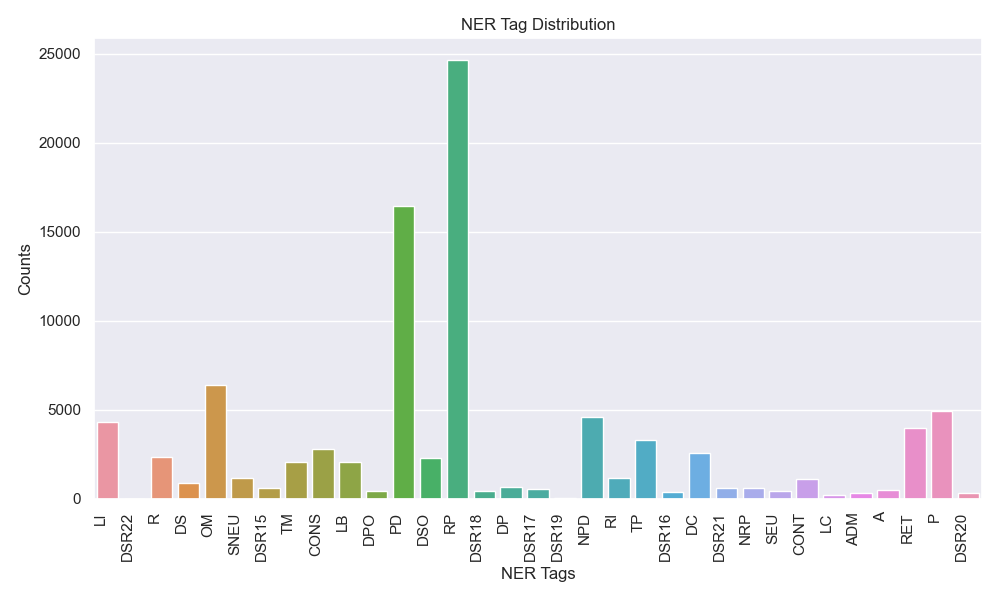
\includegraphics[width=0.99\textwidth]{images/tag_distribution.png}
    \caption{The number of occurrences of each NER tag in the annotated data set.}
    \label{fig:tag_distribution}
\end{figure*}

\subsection{Annotation guidelines}

\begin{enumerate}
    \item \textbf{Data Controller}: The individual or organization that decides (or controls) the purpose(s) of processing personal data. (E.g., \textit{This document states the OpenStreetMap privacy policy for services formally operated and provided by the \textbf{OpenStreetMap Foundation (OSMF)}.})
    
    \item \textbf{Data Processor}: A \textit{processor} means a natural or legal person, public authority, agency, or other body that processes personal data on behalf of the controller. (E.g., \textit{We may share your data with \textbf{analytics providers}, which helps us understand how customers are using our services.})
    
    \item \textbf{Data Protection Officer}: An entity within or authorized by an organization to monitor internal compliance, inform and advise on data protection obligations, and act as a contact point for data subjects and the supervisory authority. (E.g., \textit{A copy of these can be requested from the \textbf{Data Protection Officer}.})
    
    \item \textbf{Recipient}: A recipient of personal data can be used to indicate any entity that receives personal data. This can be a Third Party, Processor (GDPR), or Controller. (E.g., \textit{The data collected on the systems will be accessible by the system administrators and the appropriate OSMF \textbf{working groups}.})

    \item \textbf{Third Party}: A \textit{third party} means a natural or legal person, public authority, agency, or body other than the data subject, controller, processor, and people who, under the direct authority of the controller or processor, are authorized to process personal data. (E.g., \textit{Cycle and Transport Map layers available via the openstreetmap.org website operated by \textbf{Gravitystorm Limited, New Malden, United Kingdom}.})
    
    \item \textbf{Authority}: An authority with the power to create or enforce laws or determine their compliance. (E.g., \textit{We may disclose your data in response to official requests (e.g., court orders, subpoenas, search warrants, national security requests, etc.) ("requests") that we receive from \textbf{government authorities} or \textbf{parties to legal proceedings}.})
    
    \item \textbf{Data Subject}: The term \textit{data subject} is specific to the GDPR but is functionally equivalent to the term \textit{individual} and the ISO/IEC term \textit{PII Principle}. (E.g., \textit{This document is mainly intended for \textbf{OpenStreetMap contributors}.})

    \item \textbf{Data Source}: \textit{Source} is the direct point of data collection; \textit{origin} would indicate the original/other points where the data originates from. (E.g., \textit{User to user messages are visible to the \textbf{sender} and recipient.})

    \item \textbf{Required Purpose}: The purpose of processing personal data required for service provision. (E.g., \textit{We also use cookies and similar technologies \textbf{to recognize and improve your use of our websites}.})
    
    \item \textbf{Not-Required Purpose}: The purpose of processing personal data is not required for service provision.
    
    \item \textbf{Processing}: The processing performed on personal data. (E.g., \textit{When you visit this website or other websites, your \textbf{browser transmits data to our server}.})
    
    \item \textbf{Non-Personal Data}: The term Non-Personal Data is provided to distinguish between Personal Data and other data, indicating which data is regulated by privacy laws. (E.g., \textit{We collect \textbf{information about your browser or application and your interaction with our website}, including (a) IP address, (b) \textbf{browser and device type}, (c) \textbf{operating system}, (d) \textbf{referring web page}, (e) \textbf{the date and time of page visits}, and (f) \textbf{the pages accessed on our websites}.})
    
    \item \textbf{Personal Data}: This definition of personal data encompasses the concepts used in GDPR Art.4-1 for \textit{personal data} and ISO/IEC 27001 for \textit{personally identifiable information (PII)}. (E.g., \textit{The \textbf{full personal name} and \textbf{residential address} of members of the organisation.})
    
    \item \textbf{Organisational Measure}: Organisational measures may consist of internal policies, organizational methods or standards, and controls and audits that controllers and processors can apply to ensure the security of personal data. (E.g., \textit{In this case, a so-called \textbf{opt-out} cookie is stored in your browser.})
    
    \item \textbf{Technical Measure}: Technical measures can be defined as the measures and controls afforded to systems and any technological aspect of an organization, such as devices, networks, and hardware. (E.g., \textit{In order to protect the security of your data during transmission, we use appropriate \textbf{encryption methods in line with the latest technology (e.g., SSL/TLS)} and secure technical systems.})
    
    \item \textbf{Legal Basis}: Legal basis (\textit{plural: legal bases}) are defined by legislations and regulations, whose applicability is usually restricted to specific jurisdictions. (E.g., \textit{The processing of this data is necessary for compliance with a \textbf{legal obligation (see GDPR article 6.1c)}.})

    \item \textbf{Consent}: Consent of the Data Subject for specified processing. (E.g., \textit{\textbf{You can stop this behaviour} by explicitly turning Gravatar support off in your account settings.})
    
    \item \textbf{Contract}: Creation, completion, fulfillment, or performance of a contract involving specified processing. (E.g., \textit{To our operations and working group personnel that have signed \textbf{confidentiality agreements}.})
    
    \item \textbf{Legitimate Interest}: Legitimate interests of a Party as justification for specified processing. (E.g., \textit{We value your privacy and strive to achieve a balance between the \textbf{legitimate interests of the OpenStreetMap project} and your interests and rights.})
    
    \item \textbf{Automated Decision Making}: Processing that involves automated decision making. (E.g., \textit{If you have consented to data processing or if a contract for data processing exists and \textbf{data processing is carried out using automated processes}.})
    
    \item \textbf{Retention}: Duration, temporal limitation, or condition on storage of personal data. (E.g., \textit{Payment details for both classes of members is retained for accounting purposes \textbf{as long as required by law}.})
    
    \item \textbf{Scale EU}: Geographic coverage of processing within the European Union. (E.g., \textit{This Section 14.2 applies only to natural persons \textbf{residing in the European Economic Area} and the United Kingdom.})
    
    \item \textbf{Scale Non-EU}: Geographic coverage of processing outside the European Union. (E.g., \textit{Map tiles are provided by \textbf{a global network} of cache servers.})
    
    \item \textbf{Right}: The right(s) applicable, provided, or expected. (E.g., \textit{We value your privacy and strive to achieve a balance between the legitimate interests of the OpenStreetMap project and \textbf{your interests and rights}.})

    \item \textbf{Lodge Complaint}: A data subject can complain to a supervisory authority if the data subject considers that the processing of personal data infringes GDPR. (E.g., \textit{You also have the right to complain to the Bavarian state commissioner for data protection.})

    \item \textbf{Data Subject Rights} (26-33):
    \begin{itemize}
        \item Art. 15 Right of access by the data subject
        \item Art. 16 Right to rectification
        \item Art. 17 Right to erasure (‘right to be forgotten’)
        \item Art. 18 Right to restriction of processing
        \item Art. 19 Notification obligation regarding rectification or erasure of personal data or restriction of processing
        \item Art. 20 Right to data portability
        \item Art. 21 Right to object
        \item Art. 22 Automated individual decision-making, including profiling
    \end{itemize}
    These \textit{Data Subject Rights} are outlined in Chapter 3 of the GDPR\footnote{\url{https://gdpr.eu/tag/chapter-3/}}.
    (E.g., \textit{If incorrect personal data are processed, you have the \textbf{right to correct them (Art. 16 GDPR)}}.)
\end{enumerate}

Table \ref{tab:corrected_rounded_entity_freq_percentage_total} shows the entity frequency table for individual tokens. This table simply states the overall frequency of tokens available in the dataset.

\begin{table}[h]
\centering
\begin{tabular}{ccc}
\hline
\textbf{Label} & \textbf{Frequency} & \textbf{Percentage} \\
\hline
PD & 4200 & 23.24\% \\
P & 2909 & 16.09\% \\
RP & 1745 & 9.65\% \\
DC & 1559 & 8.62\% \\
NPD & 955 & 5.28\% \\
TP & 942 & 5.21\% \\
CONS & 686 & 3.79\% \\
TM & 648 & 3.58\% \\
R & 585 & 3.24\% \\
DS & 510 & 2.82\% \\
LB & 419 & 2.32\% \\
DSO & 408 & 2.26\% \\
OM & 386 & 2.14\% \\
LI & 306 & 1.69\% \\
RET & 291 & 1.61\% \\
SNEU & 246 & 1.36\% \\
RI & 221 & 1.22\% \\
DP & 143 & 0.79\% \\
CONT & 129 & 0.71\% \\
A & 124 & 0.69\% \\
ADM & 109 & 0.60\% \\
SEU & 100 & 0.55\% \\
DSR17 & 84 & 0.46\% \\
DSR15 & 67 & 0.37\% \\
DPO & 58 & 0.32\% \\
DSR16 & 57 & 0.32\% \\
DSR21 & 50 & 0.28\% \\
NRP & 38 & 0.21\% \\
DSR18 & 37 & 0.20\% \\
LC & 29 & 0.16\% \\
DSR20 & 29 & 0.16\% \\
DSR19 & 4 & 0.02\% \\
DSR22 & 2 & 0.01\% \\
\hline
\textbf{Overall} & \textbf{18076} & \textbf{100.00\%} \\
\hline
\end{tabular}
\caption{Entity frequency table with percentages (\textit{rounded to two decimal places}) and overall total.}
\label{tab:corrected_rounded_entity_freq_percentage_total}
\end{table}

The privacy policies have been reviewed by two legal experts and annotated. While annotating privacy policies, the annotators ensured proper formatting, such as line and word breaks. For inter-annotator agreement, the F1-measure between the two annotators, based on a set of 20 documents, is \textbf{0.6563} while Cohen's Kappa score is \textbf{0.6412}. Although the F1-score of \textbf{0.6563} indicates moderate agreement between annotators, it does not account for chance agreement. Cohen’s Kappa, however, factors this in by underscoring the potential existence of systematic bias or inconsistencies in annotation. 

The lower score is primarily the result of discrepancies in the use of Word's comment feature rather than disagreements in labeling. The decision to utilize Word's comment feature for annotating sentences or words was influenced by the annotators' familiarity with this method. When annotators highlight text for annotation, slight inconsistencies in selecting text (\textit{including an extra space before or after a word}) can lead to discrepancies in the annotated data. These minor differences, while seemingly trivial, can affect automated processing. This affects the inter-annotator agreement scores, as it may appear that annotators disagree on the annotation of the same text when, in fact, they are aligned in their understanding but differ in their selection.

After the final annotation task, we performed a basic error analysis using Precision, Recall, and F1 scores. The results showed a precision of \textbf{0.70}, a recall of \textbf{0.62}, and an F1 score of \textbf{0.65}. To encourage further academic and practical explorations in privacy policy analysis and NER applications, our dataset is publicly accessible at the following link\footnote{\url{https://huggingface.co/datasets/PaDaS-Lab/gdpr-compliant-ner}}. The dataset follows the CoNLL-2002 \cite{tjong-kim-sang-2002-introduction} format.

% \section{Enhancing Language Model Performance through Fine-Tuning}\label{section:finetune}

% For this experiment, we have worked on improving five language models including \textit{bert-base-cased}, \textit{gpt2}, \textit{albert-base-v2}, \textit{roberta-base}, and \textit{bert-base-multilingual-cased} by fine-tuning them on the GDPR-compliant privacy policy dataset that has NER annotations. To ensure consistent and reliable results, these models were fine-tuned using the same hyperparameters (\textit{Learning rate \textbf{4e-5}, Optimizer \textbf{AdamW}}) and dataset subsets. The aim of this experiment was to identify the best model for recognizing Named Entities (NER) in complex privacy policy texts.

% In a comparative analysis of the five language models, namely \textit{bert-base-cased}\footnote{\url{https://huggingface.co/bert-base-cased}}, \textit{gpt2}\footnote{\url{https://huggingface.co/gpt2}}, \textit{albert-base-v2}\footnote{\url{https://huggingface.co/albert-base-v2}}, \textit{roberta-base}\footnote{\url{https://huggingface.co/roberta-base}}, and \textit{bert-base-multilingual-cased}\footnote{\url{https://huggingface.co/bert-base-multilingual-cased}}, the model \textit{bert-base-cased} distinctly outperforms its counterparts, registering an F1-score of \textbf{0.74}. Figure \ref{fig:bert_perf}  shows a bubble chart of the confusion matrix for the fine-tuned NER model. This chart represents the model's performance in classifying various entity types.

% Table \ref{tab:llm_perform} shows the performance of the selected five language models. This practical finding is valuable for upcoming studies and practical applications in data privacy. The resulting performance of \textit{bert-base-cased} suggests the potential for creating tools and solutions to make privacy policies more user-friendly.

% \begin{table}[h]
% \centering
% \begin{tabular}{cc}
% \hline
% \textbf{Language model} & \textbf{F1-score} \\
% \hline
% \textbf{bert-base-cased} & \textbf{0.74122} \\
% gpt2 & 0.71343 \\
% albert-base-v2 & 0.71192 \\
% roberta-base & 0.72689 \\
% bert-base-multilingual-cased & 0.73534\\
% \hline
% \end{tabular}
% \caption{F1-scores of five language models. All the language models have performance above \textbf{0.70}, with \textit{bert-base-cased} having the highest performance.}
% \label{tab:llm_perform}
% \end{table}

% \begin{figure*}
%     \centering
%         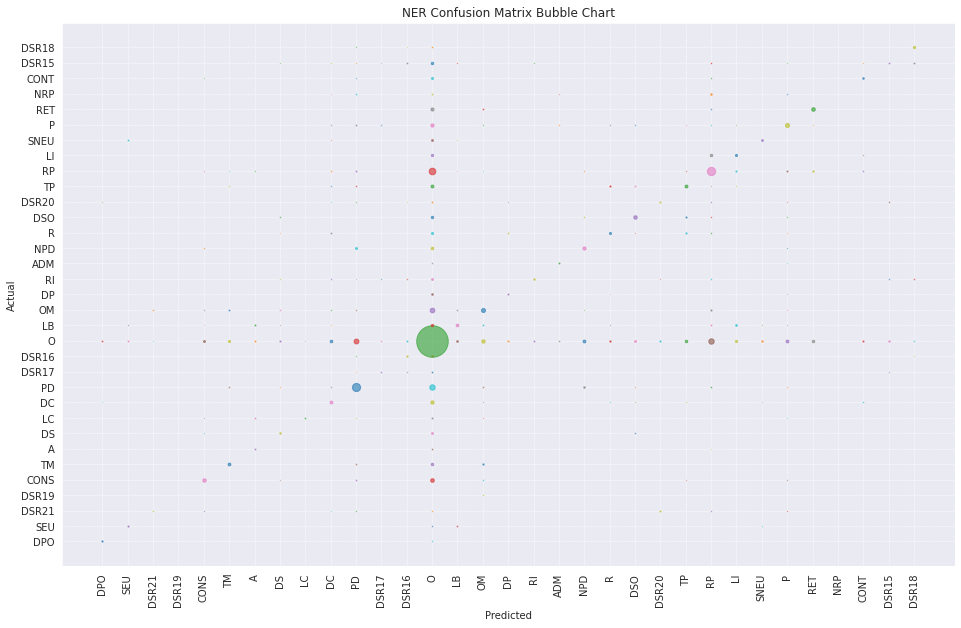
\includegraphics[width=1\textwidth]{images/ner_ed.png}
%     \caption{Each cell in this confusion matrix represents the count of instances where a particular entity type (\textit{as represented by rows}) is predicted as another type (\textit{as represented by columns}). It's important to note that the "\textit{O}" tag, representing words that are not part of any named entity,  dominates the confusion matrix due to its high occurrence in the dataset.}
%     \label{fig:bert_perf}
% \end{figure*}

\section{Conclusion}

In this study, we present a dataset enriched with Named Entity Recognition (NER) annotations that comply with GDPR. It is designed to enhance the readability and accessibility of privacy policies from 44 online platforms. The Cohen's Kappa of \textbf{0.64} reflects the reliability and consistency of the annotation process but may be influenced by sentence segmentation variations.
This dataset is a fundamental resource for the ongoing discussion on online privacy. Online data privacy presents dynamic challenges that require scrutiny, enhancements, and expansions.

This dataset lays the groundwork for future research in making privacy policies more accessible. By identifying key entities, subsequent research can focus on summarizing these policies, generating user-friendly interpretations, or creating visualization tools that simplify understanding privacy policies. Integrating Relationship Extraction (RE) could expand the dataset by capturing intricate relationships between entities and providing a more holistic understanding of privacy policies. We envision this corpus as a stepping stone towards these goals.

\section{Acknowledgments}

\begin{figure}[h]
 
\includegraphics[width=3cm]{images/BMBF.jpeg}
\end{figure} 
 The project on which this report is based was funded by the German Federal Ministry of Education and Research (BMBF) under the funding code 01|S20049, by the project DEEP WRITE (Grant No. 16DHBKI059) and the OpenWebSearch.eu project, funded by the EU under the GA 101070014.

%
% only for "biblatex"
%
\ifboolexpr{bool{jacowbiblatex}}%
	{\printbibliography}%
	{%
	% "biblatex" is not used, go the "manual" way
} % end \ifboolexpr
%
% for use as JACoW template the inclusion of the ANNEX parts have been commented out
% to generate the complete documentation please remove the "%" of the next two commands
% 
%%%\newpage

%%%\include{annexes-A4}

\end{document}
